\section{Baseline Performance Results} \label{appsec:ce}

The largest discrepancy between our and the authors' results comes from the baseline (CE) training. \cite{noisylabels-benchmark}, do not describe the exact procedure for obtaining their results. In our correspondence (see Appendix~\ref{appsec:communication}), they clarify that they used the best test set performance and report the mean and standard deviation across five random seeds. This procedure results in a discrepancy between our reproduced results and the ones reported in the original work~\citep{noisylabels-benchmark}.
We visualize the discrepancy in Figure \ref{fig:CE-difference}.  
\newline

We can see that the accuracy of the best checkpoint in our experiments is higher than their reported performance across all runs. We were not alone in noticing this discrepancy, as at the time of investigation, there were two open issues on the authors' official Github repository with the same question. Authors of the issues report the last obtained accuracies on the \textit{Worst} label set:$ \approx 68 \%$ \footnote{\url{https://github.com/UCSC-REAL/cifar-10-100n/issues/5}} and $ \approx 67 \%$ \footnote{\url{https://github.com/UCSC-REAL/cifar-10-100n/issues/8}}, which are also in line with our last epoch accuracy ($68 \pm 0.88 $).

\begin{figure}[!ht]
    \centering
    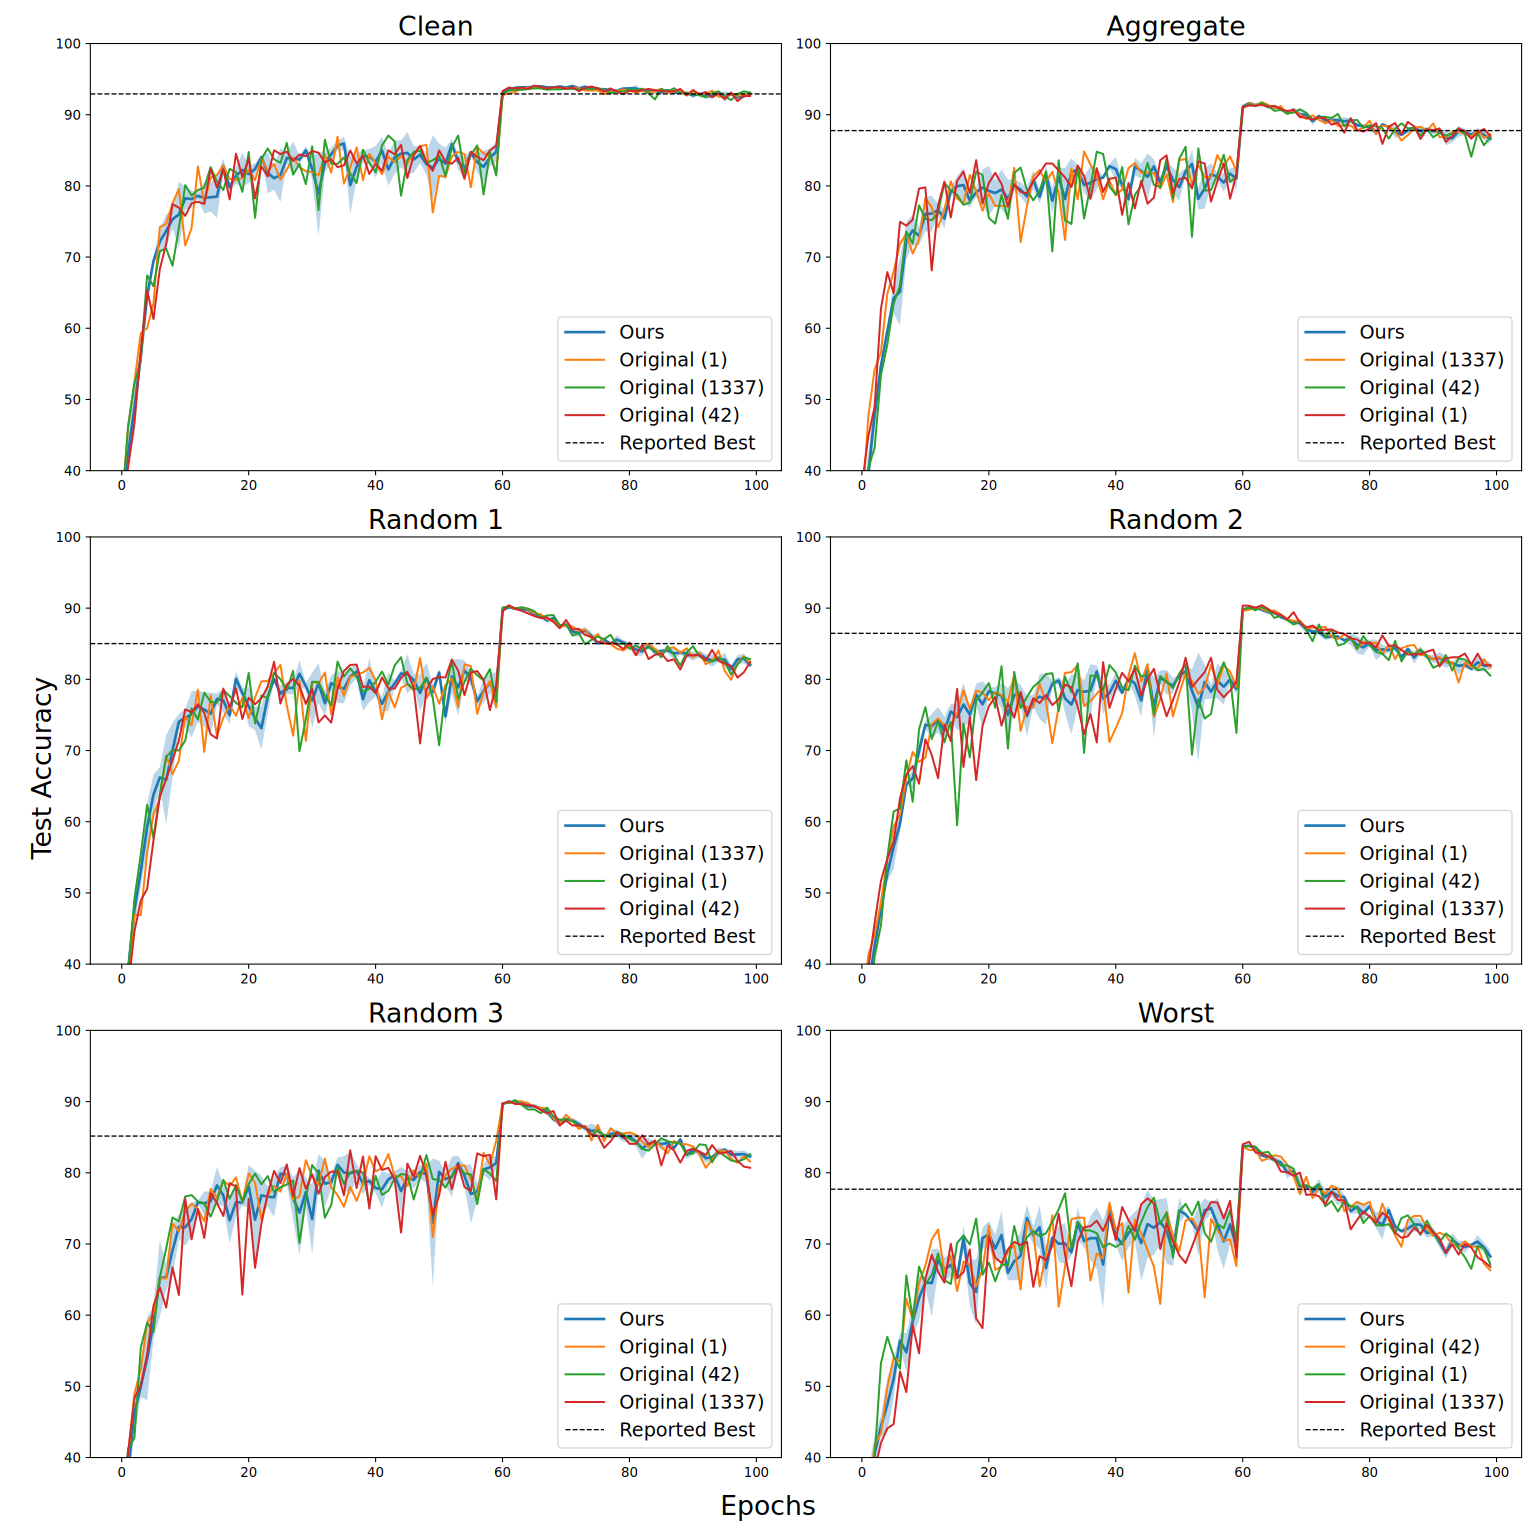
\includegraphics[width=0.8\textwidth]{figures/CE_comparison.pdf}
    \caption{\textbf{Differences between the authors' reported (dotted) baseline performance and accuracy obtained in reproduction (full blue) as well as using the original code (orange, red, green).} The performance obtained using a reimplemented framework perfectly aligns with the original code. However, on all the noise labels, their reported accuracy does not coincide with the best accuracy for any of the runs.}
    \label{fig:CE-difference}
\end{figure}


\section{Argument For Using Accuracy On Noisy Data} \label{appsec:accuracy}

% Why accuracy on clean test is not good
Since testing every epoch and reporting the highest result overestimates performance and is thus considered a bad practice, we have to find an alternative. We want to use the established train-validation-test split in this case. The first problem in LNL setting arises when we need to decide whether the validation set is noisy or not, since practices for this are not yet established in the field. Given the nature of the task, we argue that the validation set should be noisy as well~\citep{jiang2020beyond}. If one has non-noisy data, one can train on it, implicitly changing the noise ratio of the data. Additionally, some LNL methods \citep{forwardbackwardt, f-divergence} use validation data to estimate parameters for loss functions that are later used to train. If validation data were to be clean, there would be a direct data leak in such cases.
\newline

% Why we pick accuracy on noisy val
Consequently, we must decide on a proxy metric for the accuracy on clean data. We consider two options: using validation losses of each LNL method or validation accuracy. Given that losses vary between the LNL methods (some have no upper bounds) and are not as stable (see Figure~\ref{'fig:val-acc-loss'}), we propose to use accuracy on noisy validation data for model selection. We propose this, as it remains stable across all tested methods and strongly correlates with final test performance, preserving model ranking with high probability.
\newline

\begin{figure}[!ht]
    \centering
    \begin{subfigure}[t]{0.49\textwidth}
        \includegraphics[width=\linewidth]{figures/validation_loss.pdf}
        \caption{Validation loss.}
    \end{subfigure}%
    ~
    \begin{subfigure}[t]{0.49\textwidth}
        \includegraphics[width=\linewidth]{figures/validation_accuracy.pdf}
        \caption{Validation accuracy.}
    \end{subfigure}
    
    \caption{\textbf{Validation performance on noisy labels} from our benchmark implementations on the \textit{Worst} label set. 
    Some methods may assign near-zero probabilities to noisy labels, and due to the unbounded nature of the cross-entropy loss, this leads to high and unstable loss values (a). However, noisy validation accuracy remains stable across runs and serves as a reliable predictor of clean test-set performance (b). }
    \label{'fig:val-acc-loss'}
\end{figure}

% Empirical support for using noisy val
We verify our claims empirically by testing how well our approach ranks the models in comparison to the rankings of their best test set accuracies. For each method, we select the best performance on the test data and the test performance corresponding to the best validation checkpoint. We average the results across three runs and compute the Kendall rank correlation coefficient~\citep{kendall_tau} for method rankings.  For all label sets we obtain statistically significant results, indicating a strong relationship between the ordering based on noisy validation accuracy and clean test set performance. We report all the orderings with their corresponding p-value and Kendall-$\tau$ statistics below, where we underline all changes in rank:

\begin{mdframed}
{
\small
    \begin{itemize}
       \item[]CIFAR 100 - \textit{Clean} ($\tau= 1.00$, $p= 5.01e-08$)
     \item [Val:] DivideMix, ELR+, SOP+, PES semi, CE, ELR, CAL, Co-Te., Co-Te.+, SOP, VolMinNet
     \item [Test:] DivideMix, ELR+, SOP+, PES semi, CE, ELR, CAL, Co-Te., Co-Te.+, SOP, VolMinNet
    
        \item[]CIFAR 100N - \textit{Noisy} ($\tau= 1.00$, $p= 5.01e-08$)
     \item [Val:] DivideMix, PES semi, ELR+, SOP+, CE, ELR, CAL, Co-Te.+, Co-Te., VolMinNet, SOP
     \item [Test:] DivideMix, PES semi, ELR+, SOP+, CE, ELR, CAL, Co-Te.+, Co-Te., VolMinNet, SOP
    \end{itemize}
}
\end{mdframed}

\begin{mdframed}
{
\small
    \begin{itemize}
     \item[]CIFAR 10 - \textit{Clean} ($\tau= 1.0$, $p= 5.01e-08$)
     \item [Val:] SOP+, DivideMix, ELR+, PES semi, Co-Te.+, Co-Te., CE, ELR, CAL, VolMinNet, SOP
     \item [Test:] SOP+, DivideMix, ELR+, PES semi, Co-Te.+, Co-Te., CE, ELR, CAL, VolMinNet, SOP
    
     \item[]CIFAR 10N - \textit{Aggregate} ($\tau= 0.82$, $p= 1.32e-04$)
     \item [Val:] SOP+, DivideMix, ELR+, \underline{PES semi, Co-Te}, Co-Te.+, ELR, CE, CAL, VolMinNet, SOP
     \item [Test:] SOP+, DivideMix, ELR+, \underline{Co-Te., PES semi}, Co-Te.+, ELR, CE, CAL, VolMinNet, SOP
    
    
      \item[]CIFAR 10N - \textit{Random 1} ($\tau= 0.6$, $p= 9.95e-03$)
     \item [Val:] DivideMix, SOP+, PES semi, ELR+, \underline{Co-Te., ELR, Co-Te.+}, CE, CAL, SOP, VolMinNet
     \item [Test:] DivideMix, SOP+, PES semi, ELR+, \underline{Co-Te., Co-Te.+, ELR}, CE, CAL, SOP, VolMinNet
    
      \item[]CIFAR 10N - \textit{Random 2} ($\tau= 1.0$, $p= 5.01e-08$)
     \item [Val:] DivideMix, SOP+, PES semi, ELR+, Co-Te., Co-Te.+, ELR, CE, CAL, SOP, VolMinNet
     \item [Test:] DivideMix, SOP+, PES semi, ELR+, Co-Te., Co-Te.+, ELR, CE, CAL, SOP, VolMinNet
    
       \item[]CIFAR 10N - \textit{Random 3} ($\tau= 0.64$, $p= 5.71e-03$)
     \item [Val:] DivideMix, SOP+, \underline{ELR+, PES semi}, Co-Te., Co-Te.+, ELR, CE, CAL, \underline{SOP, VolMinNet}
     \item [Test:] DivideMix, SOP+, \underline{PES semi, ELR+}, Co-Te., Co-Te.+, ELR, CE, CAL, \underline{VolMinNet, SOP}
    
     
      \item[]CIFAR 10N - \textit{Worst} ($\tau= 1.0$, $p= 5.01e-08$)
     \item [Val:] DivideMix, SOP+, PES semi, ELR+, ELR, Co-Te.+, Co-Te., CE, CAL, VolMinNet, SOP
     \item [Test:] DivideMix, SOP+, PES semi, ELR+, ELR, Co-Te.+, Co-Te., CE, CAL, VolMinNet, SOP
    \end{itemize}
}
\end{mdframed} 


\citet{yuan2024early} propose LabelWave, a model selection criterion for training with noisy labels that eliminates the need for a validation set. We consider LabelWave a promising alternative to our current model selection strategy based on noisy validation accuracy. Benchmarking existing LNL methods using LabelWave as the selection criterion represents an interesting and valuable direction for future work.



\section{Additional Memorization Experiments} \label{appsec:memorization}



We extend the memorization experiments to include a broader range of synthetic noise types and hyperparameter configurations. These experiments follow the procedure described in Section~\ref{sec:noise-memorization}.



To evaluate the effect of different types of synthetic noise, we replace the asymmetric transition matrix used in Section~\ref{sec:results-memorization} with symmetric and pair-flipping noise matrices. The transition matrices are constructed following the definitions in~\cite{coteaching}, and the overall noise rate $\rho$ is estimated from the corresponding real-world noisy labels.
\newline

For symmetric noise, we set the diagonal elements of the transition matrix to $1-\rho$ and all off-diagonal elements to $\frac{\rho}{C-1}$, where $C$ is the number of classes. 
For pair-flipping noise, we again set the diagonal entries to $1-\rho$, and assign the entire off-diagonal mass $\rho$ to the most common transition class observed in the real-world noise.
\newline

 We present the results in Figure \ref{fig:memo-new-noises}. While synthetic noise types lead to varying memorization behaviors, we observe that the models still overfit human noisy labels faster than synthetic ones.



\begin{figure}[!ht]
    \centering
     
    \begin{subfigure}[b]{0.9\textwidth}
         \centering
         \includegraphics[width=\textwidth]{figures/memo_pairflip.pdf}
         \caption{} %Pair-flippin
         \label{subfig:memo-pairflip}
     \end{subfigure}
    \begin{subfigure}[b]{0.9\textwidth}
         \centering
         \includegraphics[width=\textwidth]{figures/memo_symmetric.pdf}
         \caption{} %Symmetric
         \label{subfig:memo-symmetric}
    \end{subfigure}
    \caption{\textbf{Effects of different types of synthetic noise on memorization}. (a) Pair-flipping noise constructed based on the most common transitions observed in human-labeled data. (b) Symmetric noise applied uniformly across all incorrect classes.
    In both cases, models begin to memorize human-labeled noise earlier than synthetic noise, despite different memorization dynamics.}
    \label{fig:memo-new-noises}
\end{figure}


We also investigate how different training hyperparameters influence memorization dynamics. Building on the setup described in Section~\ref{sec:noise-memorization}, we vary one hyperparameter at a time while keeping the others fixed.
\newline

In the first experiment, we replace the exponential learning rate decay with a step decay, reducing the learning rate by a factor of $\gamma=0.1$ at epoch 50. In the second experiment, we increase the initial learning rate to 0.1. In the third, we raise the weight decay to $5e-4$.
\newline

The results, shown in Figure~\ref{fig:memo-new-hparams}, indicate that while these hyperparameter changes do affect memorization behavior, the model still consistently memorizes real-world human label noise faster than synthetic noise. 
This further supports our conclusion that human-labeled, instance-dependent noise is inherently more susceptible to early memorization than instance-independent synthetic noise.
\newline

\begin{figure}[!ht]
    \centering
    \centering
    \begin{subfigure}[b]{0.9\textwidth}
         \centering
         \includegraphics[width=\textwidth]{figures/memo_step_scheduler.pdf}
         \caption{Step learning rate scheduler with a decay at epoch 50.} % Step scheduler
          \label{subfig:memo-step}
     \end{subfigure}
    \begin{subfigure}[b]{0.9\textwidth}
         \centering
         \includegraphics[width=\textwidth]{figures/memo_learning_rate.pdf}
         \caption{Lower initial learning rate set to $0.1$.} %Lower learning rate
          \label{subfig:memo-lr}
     \end{subfigure}
     \begin{subfigure}[b]{0.9\textwidth}
         \centering
         \includegraphics[width=\textwidth]{figures/memo_weight_decay.pdf}
         \caption{Increased weight decay set to $5e-4$.} %Higher weight decay
          \label{subfig:memo-wd}
     \end{subfigure}
     
      \caption{
      \textbf{Effect of hyperparameters on memorization.} We observe different memorization dynamics across hyperparameter setups. However, models consistently memorize human-labeled noise earlier than synthetic noise
      }
    \label{fig:memo-new-hparams}
\end{figure}



\section{Comments on Reproducibility} \label{appsec:reproducibility}

In this section, we document our efforts to reproduce the key experiments by~\cite{noisylabels-benchmark}, highlighting both successes and challenges. Table~\ref{tab:reproducibility} summarizes the classification of reproducibility outcomes, indicating where discrepancies arose. We also detail our communication with the original authors, the aspects of the reproduction process that were straightforward, and the challenges we faced, particularly regarding undocumented hyperparameters, inconsistent training protocols, and unclear benchmarking procedures.

\begin{table}[!ht]

    \caption{\textbf{Classification of reproducibility results.}}
    \centering
    { \footnotesize
    \begin{tabular}{ccc}
        \toprule
        Experiment & Discrepancy & Result\\
        \midrule
        Noise hypothesis testing & Missing details in experimental setup. & Reproduced \\
        Memorization effects  & Missing details in experimental setup.  & Reproduced \\
        Baseline performance & Difference in reported vs. observed results. & Different\\
        LNL Benchmark &Ambiguities in paper descriptions. & Reimplemented\\
        \bottomrule
    \end{tabular}
    }
    \label{tab:reproducibility}
\end{table}



\subsection{Communication with Original Authors}
\label{appsec:communication}

We contacted the authors two times during our implementation effort. The first time, we inquired about several inconsistencies between the paper and the provided code. We also asked about the hyperparameter selection protocol, which backbone models were used, which checkpoints were selected, and some general evaluation and method-specific questions. The authors responded with a short email, answering some of our questions but avoiding our questions about inconsistencies.
\newline

After some time, we contacted the authors for the second time. We inquired how the validation sets were handled, as some methods could not be properly trained without them. We also asked about the specifics of the hypothesis testing setup and the differences between the original and our reproduced results. This time, the authors did not respond.

\subsection{What was easy}

Using the baseline code and the datasets provided by the benchmark authors was easy and only required minimal tweaking to run. Running most of the LNL strategies' repositories was also straightforward, as most authors include instructions for basic use cases and experiment reproduction in the source code repository.

\subsection{What was difficult}

Throughout the reproduction attempt, we encountered several problems, most of them stemming from unclear and ambiguous descriptions of the benchmark. Many evaluated methods rely on algorithm-specific hyperparameters, which the authors did not list. Therefore, an effort was made to try to recover them by experimentally trying out different combinations in an attempt to match the reported results. The learning rate schedule for all methods was said to follow a multi-step schedule with a single decay at the 50th epoch. In the original source code, the switch happens at the 60th epoch. 

Several LNL methods use different warm-up training techniques. Some fully reset the model, while others use the warm-up epochs to find a set of weights that perform best on the validation set and later continue the training from the pre-trained checkpoint. A shared checkpoint was supposed to be used for the benchmark. However, the paper does not mention how such a checkpoint was obtained. After communication with the authors, they clarified that the warmup checkpoint was obtained by training the model with cross-entropy loss for 200 epochs.


\section{Computational Requirements} 
\label{appsec:computational-requirements}

We run all our experiments on a system with $8$ Nvidia Titan X Pascal GPUs running Ubuntu 20.04.2 LTS and CUDA version 12.2.
With this setup, it takes approximately $1.5$ GPU hours to reproduce the noise hypothesis testing experiment and approximately $27$ GPU hours to reproduce the noise memorization experiment.
Reproducing benchmark results on the selected subset of the LNL methods takes approximately $52.5$ GPU hours per label set; we present a breakdown of the training times in Table~\ref{tab:runtimes}.
It takes approximately $2,000$ GPU hours to reproduce our results fully (eight label sets, each with three repeats, and six synthetic runs with two repeats).

\begin{table}[!ht]
\centering
\caption{\textbf{Runtimes of the 10 selected methods}, for a single repeat of a single noise label.}
{ \footnotesize
\begin{tabular}{l r}
\toprule
\textbf{Method} & \textbf{Runtime (h)} \\
\midrule
CE & $1.5$ \\
Co-teaching (+) & $5.6$ \\
ELR & $1.8$ \\
ELR+ & $7.9$ \\
DivideMix & $14.0$ \\
VolMinNet & $1.3$ \\
CAL & $1.5$ \\
PES (semi) & $12.2$ \\
SOP+ & $5.5$ \\
SOP & $1.2$ \\
\hline
total & $52.5$ \\
\bottomrule
\end{tabular}
}
\label{tab:runtimes}
\end{table}

\section{Hyperparameters} \label{appsec:hyperparams}

In this section, we report the hyperparameters for all the methods included in our reproduced evaluation to enable the replication of our results. Table~\ref{tab:hyperPreact} describes the hyperparameters of methods using the \textit{PreActResNet18}~\citep{preact} backbone, and Table~\ref{tab:hyper34} for the methods using the \textit{ResNet-34}~\citep{he2015resnet} backbone. Here we note that most of the methods' original implementations as well as the model implementation provided by the authors~\footnote{\url{https://github.com/UCSC-REAL/cifar-10-100n/blob/main/models/resnet.py}} use ResNet implementations that use stride of $1$ instead of $2$ in the first layer, resulting in a four times increase in activation volumes. The modified implementation also excludes the first max pooling layer (see \cite{he2015resnet} Table 1), resulting in another four-times increase in activation volumes, for a total of $16$ times bigger activation volumes. Modifying these layers increases the baseline performance significantly ($10\%$ when comparing baselines in Tables ~\ref{tab:bechmark-results} and \ref{tab:our-benchmark}).
\newline

In our reproduction experiments, we use this version of ResNet since it was provided in the author's original repository. For our benchmark (Section~\ref{sec:our-benchmark}) we use the same hyperparameters as described in tables \ref{tab:hyper34} and \ref{tab:hyperPreact} with the exception of using the official PyTorch implementation of ResNet~\footnote{\url{https://pytorch.org/vision/main/models/resnet.html}}.
We report the parameters for newer methods not used in the original benchmark: DISC and ProMix in Table~\ref{tab:hyper-sota}.



\begin{table}[p]
    \centering
    \caption{Hyperparameters for newer methods.}
    { \scriptsize
        
\begin{tabular}{ll|cc}
    \toprule
    Method & Hyperparameter & CIFAR10N & CIFAR100N \\
    \midrule
    \multirow{12}{*}{DISC} & optimizer & SGD & SGD \\
     & lr & 0.1 & 0.1 \\
     & weight\_decay & 0.001 & 0.001 \\
     & SGD momentum & 0 & 0 \\
     & scheduler & MultiStepLR ([80, 160], 0.1)& MultiStepLR ([80, 160], 0.1) \\
     & epochs & 200 & 200 \\
     & alpha & 5.0 & 5.0 \\
     & start\_epoch & 15 & 15 \\
     & sigma & 0.5 & 0.5 \\
     & momentum & 0.99 & 0.99 \\
     & lambda\_ce & 1.0 & 1.0 \\
     & lambda\_h & 1.0 & 1.0 \\
    \hline
    \multirow{18}{*}{ProMix} & optimizer & SGD & SGD \\
     & lr & 0.05 & 0.05 \\
     & weight\_decay & 0.0005 & 0.0005 \\
     & momentum & 0.9 & 0.9 \\
     & scheduler & CosineAnnealingLR & CosineAnnealingLR\\
     & epochs & 600 & 600 \\
     & warmup\_epochs & 10 & 30 \\
     & rampup\_epochs & 50 & 50 \\
     & noise\_type & symmetric & symmetric \\
     & rho\_start, rho\_end & (0.5, 0.5) & (0.5, 0.5) \\
     & debias\_beta\_pl & 0.8 & 0.5 \\
     & alpha\_output & 0.8 & 0.5 \\
     & tau & 0.99 & 0.95 \\
     & start\_expand & 250 & 250 \\
     & threshold & 0.9 & 0.9 \\
     & bias\_m & 0.9999 & 0.9999 \\
     & temperature 0.5 & 0.5 \\
     & feat\_dim & 128 & 128 \\
     \bottomrule
\end{tabular}

    }

    \label{tab:hyper-sota}
\end{table}

\begin{table}[p]
    \centering
    \caption{Hyperparameters for methods using PreActResNet18 backbone.}
    { \scriptsize
        \begin{tabular}{lccc}
\toprule
Method & Hyperparameter & CIFAR10N & CIFAR100N \\
\midrule
\multirow{12}{*}{DivideMix} & optimizer & SGD & SGD \\
 & lr & 0.02 & 0.02 \\
 & weight\_decay & 0.0005 & 0.0005 \\
 & momentum & 0.9 & 0.9 \\
 & scheduler & LambdaLR & LambdaLR \\
 & epochs & 300 & 300 \\
 & alpha & 4 & 4 \\
 & noise\_type & asymmetric & asymmetric \\
 & p\_thresh & 0.5 & 0.5 \\
 & temperature & 0.5 & 0.5 \\
 & lambda\_u & 0 & 0 \\
 & warmup\_epochs & 10 & 30 \\
\hline
\multirow{12}{*}{ELR+} & optimizer & SGD & SGD \\
 & lr & 0.02 & 0.02 \\
 & weight\_decay & 0.0005 & 0.0005 \\
 & momentum & 0.9 & 0.9 \\
 & scheduler & MultiStepLR ([150], 0.1) & MultiStepLR ([200], 0.1) \\
 & epochs & 200 & 250 \\
 & beta & 0.7 & 0.9 \\
 & lmbd & 3 & 7 \\
 & alpha & 1 & 1 \\
 & gamma & 0.997 & 0.997 \\
 & ema\_step & 40000 & 40000 \\
 & coef\_step & 0 & 40000 \\
\hline
\multirow{12}{*}{SOP+} & optimizer & SGD & SGD \\
 & lr & 0.02 & 0.02 \\
 & weight\_decay & 0.0005 & 0.0005 \\
 & momentum & 0.9 & 0.9 \\
 & scheduler & CosineAnnealing & CosineAnnealing \\
 & epochs & 300 & 300 \\
 & lr\_u & 10 & 1 \\
 & lr\_v & 10 & 10 \\
 & overparam\_mean & 0.0 & 0.0 \\
 & overparam\_std & 1e-08 & 1e-08 \\
 & ratio\_balance & 0.1 & 0.1 \\
 & ratio\_consistency & 0.9 & 0.9 \\
\bottomrule
\end{tabular}


    }

    \label{tab:hyperPreact}
\end{table}

\begin{table}[p]
    \centering
    \caption{Hyperparameters for methods using ResNet-34 backbone.}
    { \tiny
        \begin{tabular}{lccc}
\toprule
Method & Hyperparameter & CIFAR-10N & CIFAR-100N \\
\midrule
\multirow{13}{*}{CAL} & optimizer & SGD & SGD \\
 & lr & 0.1 & 0.1 \\
 & weight\_decay & 0.0005 & 0.0005 \\
 & momentum & 0.9 & 0.9 \\
 & scheduler & MultiStepLR ([60], 0.1) & MultiStepLR ([60], 0.1) \\
 & epochs & 165 & 165 \\
 & alpha & 0.0 & 0.0 \\
 & alpha\_scheduler & seg & seg \\
 & warmup\_epochs & 65 & 65 \\
 & alpha\_list\_warmup & [0.0, 2.0] & [0.0, 1.0] \\
 & milestones\_warmup & [10, 40] & [10, 40] \\
 & alpha\_list & [0.0, 1.0, 1.0] & [0.0, 1.0, 1.0] \\
 & milestones & [10, 40, 80] & [10, 40, 80] \\
\hline
\multirow{6}{*}{CE} & optimizer & SGD & SGD \\
 & lr & 0.1 & 0.1 \\
 & weight\_decay & 0.0005 & 0.0005 \\
 & momentum & 0.9 & 0.9 \\
 & scheduler & MultiStepLR ([60], 0.1) & MultiStepLR ([60], 0.1) \\
 & epochs & 100 & 100 \\
\hline
\multirow{9}{*}{Co-teaching} & optimizer & Adam & Adam \\
 & lr & 0.001 & 0.001 \\
 & weight\_decay & 0 & 0 \\
 & scheduler & alpha\_schedule & alpha\_schedule \\
 & epochs & 200 & 200 \\
 & forget\_rate & 0.2 & 0.2 \\
 & exponent & 1 & 1 \\
 & num\_gradual & 10 & 10 \\
 & epoch\_decay\_start & 80 & 100 \\
\hline
\multirow{10}{*}{Co-teaching+} & optimizer & Adam & Adam \\
 & lr & 0.001 & 0.001 \\
 & weight\_decay & 0 & 0 \\
 & scheduler & alpha\_schedule & alpha\_schedule \\
 & epochs & 200 & 200 \\
 & init\_epoch & 20 & 5 \\
 & forget\_rate & 0.2 & 0.2 \\
 & exponent & 1 & 1 \\
 & num\_gradual & 10 & 10 \\
 & epoch\_decay\_start & 80 & 80 \\
\hline
\multirow{8}{*}{ELR} & optimizer & SGD & SGD \\
 & lr & 0.02 & 0.02 \\
 & weight\_decay & 0.001 & 0.001 \\
 & momentum & 0.9 & 0.9 \\
 & scheduler & CosineAnnealing & MultiStepLR ([80, 120], 0.01) \\
 & epochs & 120 & 150 \\
 & beta & 0.7 & 0.9 \\
 & lmbd & 3 & 7 \\
\hline
\multirow{12}{*}{PES (semi)} & optimizer & SGD & SGD \\
 & lr & 0.02 & 0.02 \\
 & weight\_decay & 0.0005 & 0.0005 \\
 & momentum & 0.9 & 0.9 \\
 & scheduler & CosineAnnealing & CosineAnnealing \\
 & epochs & 300 & 300 \\
 & PES\_lr & 0.0001 & 0.0001 \\
 & warmup\_epochs & 20 & 35 \\
 & T2 & 5 & 5 \\
 & lambda\_u & 5 & 75 \\
 & temperature & 0.5 & 0.5 \\
 & alpha & 4 & 4 \\
\hline
\multirow{12}{*}{SOP} & optimizer & SGD & SGD \\
 & lr & 0.02 & 0.02 \\
 & weight\_decay & 0.0005 & 0.0005 \\
 & momentum & 0.9 & 0.9 \\
 & scheduler & MultiStepLR ([40, 80], 0.1) & MultiStepLR ([40, 80], 0.1) \\
 & epochs & 120 & 150 \\
 & lr\_u & 10 & 1 \\
 & lr\_v & 10 & 10 \\
 & overparam\_mean & 0.0 & 0.0 \\
 & overparam\_std & 1e-08 & 1e-08 \\
 & ratio\_balance & 0.0 & 0.0 \\
 & ratio\_consistency & 0.0 & 0.0 \\
\hline
\multirow{9}{*}{VolMinNet} & optimizer & SGD & SGD \\
 & lr & 0.01 & 0.01 \\
 & weight\_decay & 0.0001 & 0.0001 \\
 & momentum & 0.9 & 0.9 \\
 & scheduler & MultiStepLR ([30, 60], 0.1) & MultiStepLR ([30, 60], 0.1) \\
 & epochs & 80 & 80 \\
 & lam & 0.0001 & 0.0001 \\
 & init\_t & 2 & 2 \\
 & optimizer\_transition\_mtx & SGD & Adam \\
\bottomrule
\end{tabular}
    }

    \label{tab:hyper34}
\end{table}

\end{document}
